% !TeX root=../main.tex
\chapter{روش تحقیق}

\section{مقدمه و نمای کلی روش پیشنهادی}
\label{sec:ch3-intro}
در این فصل روشی برای طبقه‌بندی چندکلاسه با بهره‌گیری از ساختار ارتباطی نمونه‌ها و ویژگی‌های آن‌ها معرفی می‌شود. ایده محوری آن است که به‌جای استخراج یک بازنمایی یکسان برای تمام تصمیم‌های کلاسی، برای هر فرضیه تعلق به یک کلاس، سیاست انتخاب ویژگی مستقلی آموخته شود. این سیاست نحوه حرکت روی گراف داده‌ها را تعیین می‌کند؛ مشاهدات برچسبی حاصل از حرکت نیز به یک توزیع احتمال تبدیل می‌شوند. سپس با مقایسه بازنمایی نمونه با مراکز کلاسی متناظر با همان سیاست، میزان سازگاری آن نمونه با فرضیه مورد بررسی سنجیده می‌شود.

\subsection{انگیزه و ایده اصلی روش}
\label{subsec:ch3-motivation}
یک ویژگی ممکن است برای تشخیص یک کلاس از سایر کلاس‌ها مفید باشد، ولی برای فرضیه کلاسی دیگری اهمیت کمتری داشته باشد. از سوی دیگر، حضور نداشتن بعضی ویژگی‌ها در یک نمونه نباید به معنی مقداردهی ساختگی به آن ویژگی‌ها باشد. مدل پیشنهادی این دو ملاحظه را با ساخت یک گراف نمونه--ویژگی و تعریف سیاست‌های وابسته به فرضیه ترکیب می‌کند. گراف، ارتباط نمونه‌ها از طریق ویژگی‌های مشترک را نمایش می‌دهد و سیاست، ویژگی مورد استفاده در هر مرحله جست‌وجوی همسایگی را انتخاب می‌کند.

هدف یادگیری صرفاً نزدیک کردن بازنمایی نمونه‌های هم‌کلاس به یکدیگر نیست. یک سیاست مناسب برای فرضیه کلاس $c$ باید بتواند نمونه‌های متعلق به $c$ را بپذیرد و نمونه‌های متعلق به کلاس‌های دیگر را رد کند. بنابراین کیفیت سیاست در نهایت از دیدگاه خطاهای آزمون فرضیه بررسی می‌شود، نه فقط بر اساس جدایی مراکز بازنمایی.

\subsection{سیاست‌های وابسته به فرضیه‌های کلاسی}
\label{subsec:ch3-hypothesis-policies}
اگر مجموعه کلاس‌ها $\mathcal C=\{1,\ldots,K\}$ باشد، برای هر $c\in\mathcal C$ سیاست $\pi^{(c)}$ تعریف می‌کنیم. این سیاست روی \emph{تمام نمونه‌ها}، چه متعلق به کلاس $c$ باشند و چه نباشند، قابل اجراست. بازنمایی حاصل را با $P_X^{(c)}$ نشان می‌دهیم. ازاین‌رو برای یک نمونه واحد ممکن است $K$ بازنمایی متفاوت تولید شود که هر کدام شواهد مربوط به یک فرضیه کلاسی را منعکس می‌کنند.

پارامترهای هر سیاست در میان نمونه‌ها مشترک‌اند؛ در نتیجه روش پیشنهادی برای هر زوج نمونه--ویژگی، مجموعه پارامتر جداگانه‌ای یاد نمی‌گیرد. با این حال، در هر نمونه، ویژگی‌های ناموجود یا انتقال‌های ممنوع از مجموعه گزینه‌های قابل انتخاب کنار گذاشته می‌شوند.

\subsection{نمای کلی مراحل آموزش و پیش‌بینی}
\label{subsec:ch3-overview}
فرایند روش پیشنهادی شامل ساخت گراف ارتباطی داده‌ها، تعیین توزیع گذار میان نمونه‌ها، تعریف سیاست انتخاب ویژگی، محاسبه بازنمایی چندگامی و تشکیل مراکز کلاس‌هاست. پس از آن، برای هر فرضیه، یک امتیاز سازگاری مبتنی بر اختلاف واگرایی‌ها ساخته می‌شود و سیاست با هدف کاهش پذیرش نادرست نمونه‌های منفی در سطح مشخصی از رد نادرست نمونه‌های مثبت آموزش می‌بیند. در زمان پیش‌بینی، برچسب نمونه پرس‌وجو در دسترس نیست؛ ازاین‌رو تمام سیاست‌ها مستقل از برچسب واقعی آن اجرا می‌شوند و نتیجه هر آزمون با آستانه کالیبره‌شده همان فرضیه مقایسه می‌شود. قاعده تبدیل چند نتیجه آزمون به یک برچسب نهایی، مرحله‌ای مستقل است و در انتهای فصل درباره گزینه‌های آن بحث می‌شود.

\section{صورت‌بندی مسئله و مفروضات پایه}
\label{sec:ch3-problem}
\subsection{مجموعه داده و طبقه‌بندی چندکلاسه تک‌برچسبی}
\label{subsec:ch3-dataset}
مجموعه داده آموزشی برچسب‌دار را به‌شکل
\[
\mathcal D=\{(X_i,y_i)\}_{i=1}^{n},\qquad y_i\in\mathcal C=\{1,\ldots,K\}
\]
در نظر می‌گیریم که در آن $K\ge2$ و هر نمونه دقیقاً به یک کلاس تعلق دارد. مجموعه نمونه‌های کلاس $k$ و تعداد آن‌ها به‌ترتیب با
\[
\mathcal C_k=\{i:y_i=k\},\qquad n_k=|\mathcal C_k|>0
\]
مشخص می‌شوند. تفکیک اندیس نمونه‌ها از برچسب کلاس‌ها، به‌ویژه هنگام محاسبه میانگین‌های کلاسی و محدودیت بازگشت به مبدأ ضروری است. منظور از «نمونه جدید» در زمان آزمون، نمونه‌ای است که برچسب آن معلوم نیست و نباید در ساخت شواهد برچسبی مورد استفاده قرار گیرد.

\subsection{فضای ویژگی‌ها و ویژگی‌های ناموجود}
\label{subsec:ch3-features}
مجموعه ویژگی‌های قابل استفاده را $A_D=\{a_1,\ldots,a_m\}$ و زیرمجموعه ویژگی‌های موجود در نمونه $X_i$ را $A_{X_i}\subseteq A_D$ می‌نامیم. نبود یک ویژگی با مقدار عددی صفر آن متفاوت است؛ ویژگی ناموجود اساساً در فرایند انتخاب ویژگی و انتقال متناظر شرکت نمی‌کند. برای هر ویژگی $a$، مجموعه اندیس نمونه‌هایی که آن ویژگی را دارند برابر است با
\[
I_a=\{i:a\in A_{X_i}\},\qquad D_a=\{X_i:i\in I_a\}.
\]
تعریف این مجموعه‌ها برای داده‌های دارای الگوی متفاوتی از ویژگی‌های موجود، یک مدل مشترک فراهم می‌کند؛ بدون آنکه لازم باشد مقادیر ناموجود تخمین زده شوند.

\subsection{نمادگذاری مجموعه‌ها و متغیرهای اصلی}
\label{subsec:ch3-notation}
در ادامه $s$ اندیس نمونه آغازین مسیر، $i$ و $j$ اندیس نمونه‌های گراف و $a,b$ نام ویژگی‌ها هستند. $T_a(X_j\mid X_i)$ احتمال انتقال بین نمونه‌ها از طریق ویژگی $a$، و $\pi^{(c)}(b\mid X_j,a)$ احتمال انتخاب ویژگی بعدی $b$ پس از ویژگی $a$ تحت فرضیه $c$ است. نماد $e_k$ بردار یکه مربوط به کلاس $k$ در فضای $\mathbb R^K$، نماد $P_{X_i}^{(c)}$ بازنمایی احتمالاتی نمونه، و نماد $V_{k\mid c}$ مرکز نمونه‌های کلاس واقعی $k$ در فضای بازنمایی سیاست $c$ را نشان می‌دهد. تمام توزیع‌های برچسب در سیمپلکس
\[
\Delta^{K-1}=\{p\in\mathbb R^K:p_k\ge0,\ \sum_{k=1}^Kp_k=1\}
\]
قرار دارند. پارامتر $\beta$ احتمال توقف پس از هر مشاهده و $\lambda$ ضریب وزن‌دهی به عمق مشاهدات است.

\subsection{مفروضات کفایت نمونه و وجود انتقال معتبر}
\label{subsec:ch3-assumptions}
فرض می‌کنیم وزن انتقال میان هر دو نمونه متمایز که ویژگی مشترک مورد استفاده را دارند، مثبت است. همچنین برای ویژگی‌هایی که در حرکت فعال می‌شوند، تعداد نمونه‌های دارای آن ویژگی به اندازه‌ای است که پس از حذف نمونه فعلی و ممنوعیت بازدید مجدد از مبدأ، دست‌کم یک مقصد مجاز باقی بماند. شرط ساده و کافی برای این منظور
\[
|D_a|\ge3\qquad(a\in A_D)
\]
به‌همراه مثبت بودن وزن‌های بین نمونه‌های متمایز است. در صورت برقراری این فرض، ماتریس‌های انتقال روی حالت‌های قابل دسترس تصادفی‌اند و حرکت به بن‌بست ساختاری نمی‌رسد. شرط فوق برای سادگی تحلیل ارائه شده است و در داده‌هایی که آن را نقض می‌کنند، باید پیش از اجرای مدل، ویژگی‌های نامعتبر یا مجموعه انتقال‌های مجاز تعیین تکلیف شوند.

در فرایند آموزش، هنگام ساخت بازنمایی نمونه مبدأ، بازگشت به همان نمونه در تمام مراحل مسیر ممنوع است. سایر نمونه‌ها ممکن است چند بار بازدید شوند. تصمیم‌های انتخاب ویژگی تنها بر ویژگی‌های موجود و اطلاعات مجاز متکی‌اند؛ هیچ مرحله‌ای از اجرای سیاست روی نمونه پرس‌وجو، برچسب واقعی آن را مطالبه نمی‌کند. برای محاسبه روابط مبتنی بر لگاریتم نیز در صورت نیاز از هموارسازی مثبت توزیع‌ها استفاده خواهد شد.

\section{ساخت گراف نمونه--ویژگی}
\label{sec:sample-feature-graph}
برای مدل‌سازی هم‌زمان وابستگی میان نمونه‌ها و امکان جابه‌جایی میان ویژگی‌های یک نمونه، مجموعه داده را به‌صورت یک گراف درهم‌تنیده نمونه--ویژگی نمایش می‌دهیم. در این نمایش، هر نمونه یک مجموعه از ویژگی‌های موجود خود را در اختیار دارد؛ گره‌های متناظر با یک ویژگی، امکان ارتباط میان نمونه‌ها را فراهم می‌کنند و ارتباط‌های درون یک نمونه، انتخاب ویژگی مورد استفاده در انتقال بعدی را مدل می‌کنند. این دو نوع ارتباط از نظر معنایی و احتمال گذار متمایزند.

\subsection{تعریف رأس‌ها و ساختار گراف}
\label{subsec:graph-vertices}
مجموعه داده برچسب‌دار را با
\[
D=\{(X_i,y_i)\}_{i=1}^{n}
\]
نشان می‌دهیم. مجموعه همه ویژگی‌ها را $A_D$ و مجموعه ویژگی‌های موجود برای نمونه $X_i$ را $A_{X_i}\subseteq A_D$ می‌نامیم. برای هر ویژگی $a$ نیز تعریف می‌کنیم:
\[
D_a=\{X_i:i\in I_a\}.
\]
در اینجا $I_a$ مجموعه اندیس‌های نمونه‌هایی است که ویژگی $a$ را دارند.

گراف پیشنهادی به‌صورت
\[
G=(\mathcal V,\mathcal E_{\mathrm v}\cup\mathcal E_{\mathrm h})
\]
تعریف می‌شود که در آن
\[
\mathcal V=\{(X_i,a):X_i\in D,\;a\in A_{X_i}\}.
\]
بنابراین هر رأس، یک \emph{زوج نمونه--ویژگی} است، نه صرفاً یک نمونه یا یک ویژگی. $\mathcal E_{\mathrm v}$ ارتباط‌های میان نمونه‌ها در امتداد ویژگی مشترک و $\mathcal E_{\mathrm h}$ ارتباط‌های انتخاب ویژگی درون یک نمونه را نمایش می‌دهند.

برای روشن شدن ساختار، شکل~\ref{fig:ch3-sample-feature-graph} نمای شماتیک سه نمونه با چهار ویژگی $A$، $B$، $C$ و $D$ را نشان می‌دهد. رنگ هر مسیر پیوسته به یک ویژگی تعلق دارد و گره‌های دارای اندیس یکسان به یک نمونه مربوط‌اند. گروه‌بندی گره‌ها برحسب اندیس نمونه، مرز مفهومی هر نمونه را مشخص می‌کند.

\begin{figure}[htbp]
  \centering
  % تصویر اصلی کاربر بدون بازطراحی؛ پس از افزودن PNG به مخزن، به طور خودکار نمایش داده می‌شود.
  \IfFileExists{./img/chap3/sample-feature-graph.png}{%
    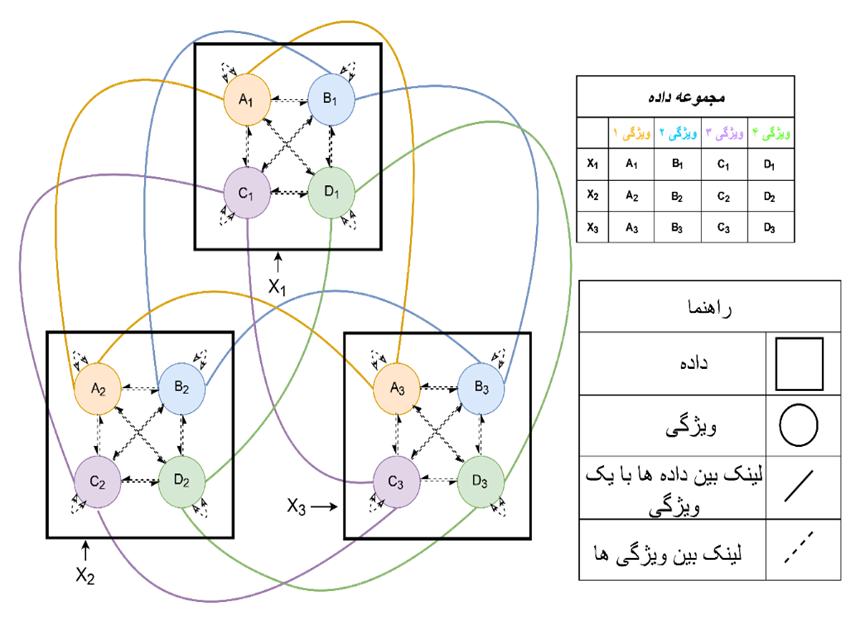
\includegraphics[width=0.94\linewidth]{./img/chap3/sample-feature-graph.png}%
  }{%
    \fbox{\parbox{0.86\linewidth}{\centering
      محل تصویر اصلی گراف نمونه--ویژگی؛ فایل \lr{img/chap3/sample-feature-graph.png} هنوز به مخزن افزوده نشده است.}}%
  }
  \caption{نمای شماتیک گراف نمونه--ویژگی برای سه نمونه و چهار ویژگی؛ یال‌های پیوسته، ارتباط بین نمونه‌ها از طریق یک ویژگی مشترک و یال‌های گسسته، ارتباط‌های درون هر نمونه را نشان می‌دهند.}
  \label{fig:ch3-sample-feature-graph}
\end{figure}

\subsection{ارتباط‌های درون نمونه و میان نمونه‌ها}
\label{subsec:graph-edge-types}
ارتباط \emph{میان‌نمونه‌ای} از رأس $(X_i,a)$ به رأس $(X_j,a)$ برقرار می‌شود، به شرط آنکه $i\ne j$، ویژگی $a$ در هر دو نمونه موجود باشد و وزن ارتباط مجاز باشد. این ارتباط امکان انتقال از یک نمونه به نمونه دیگر \emph{بدون تغییر ویژگی مبنای انتقال} را فراهم می‌کند. در شکل، این یال‌ها به‌صورت مسیرهای پیوسته هم‌رنگ ترسیم شده‌اند. مفهوم جهت‌داری انتقال به‌صورت احتمالات گذار تعریف می‌شود و الزاماً از شکل ظاهری منحنی‌ها قابل استنتاج نیست.

در مقابل، ارتباط \emph{درون‌نمونه‌ای} از $(X_i,a)$ به $(X_i,b)$ برای ویژگی‌های موجود $a,b\in A_{X_i}$ تعریف می‌شود. این ارتباط‌ها \emph{جهت‌دار} هستند: انتخاب $b$ پس از $a$ لزوماً همان وزن یا احتمال انتخاب $a$ پس از $b$ را ندارد. همچنین حالت $a=b$ مجاز است؛ ازاین‌رو هر ویژگی موجود می‌تواند دارای \emph{طوقه} باشد و سیاست می‌تواند در گام بعد همان ویژگی را دوباره انتخاب کند. در نمایش شماتیک، خطوط گسسته روابط درون‌نمونه‌ای را نشان می‌دهند، اما تمام جهت‌ها، وزن‌های مستقل و طوقه‌ها لزوماً در شکل رسم نشده‌اند.

این تفکیک از آن جهت اهمیت دارد که یک گام حرکت پیشنهادی از دو تصمیم تشکیل می‌شود: نخست انتخاب ویژگی بعدی با استفاده از سیاست درون‌نمونه‌ای، و سپس انتقال به نمونه‌ای دیگر از طریق ویژگی انتخاب‌شده. بنابراین یال میان‌نمونه‌ای و انتخاب ویژگی دو مفهوم متفاوت هستند و نباید با یک احتمال واحد جایگزین شوند.

\subsection{وزن شباهت و احتمالات انتقال بین نمونه‌ها}
\label{subsec:graph-similarity}
برای ویژگی $a$، وزن غیرمنفی
$w_a(X_i,X_j)$
میزان ارتباط نمونه‌های $X_i$ و $X_j$ را بر اساس آن ویژگی مشخص می‌کند. اگر $X_i$ مبدأ انتقال باشد، احتمال انتخاب مقصد $X_j$ با نرمال‌سازی وزن‌های مجاز به دست می‌آید:
\[
T_a(X_j\mid X_i)=
\frac{w_a(X_i,X_j)}
{\displaystyle\sum_{\substack{X_\ell\in D_a\\\ell\ne i}}w_a(X_i,X_\ell)},
\qquad X_j\in D_a,\ j\ne i.
\]
این رابطه تنها هنگامی به کار می‌رود که مخرج مثبت باشد. شیوه محاسبه وزن‌ها و جزئیات محدودیت‌های وابسته به مبدأ در ادامه روش مشخص خواهند شد. به‌طور کلی لازم نیست $T_a(X_j\mid X_i)$ و $T_a(X_i\mid X_j)$ برابر باشند؛ حتی در صورت تقارن وزن‌های خام، نرمال‌سازی در مبدأهای متفاوت ممکن است احتمال‌های متفاوتی ایجاد کند.

\subsection{محدودیت‌های انتقال و کنار گذاشتن نمونه مبدأ}
\label{subsec:graph-transition-constraints}
در داده‌های واقعی ممکن است بعضی ویژگی‌ها برای یک نمونه ناموجود باشند. برای نمایش شهودی، می‌توان محل چنین ویژگی‌هایی را با دایره توخالی نشان داد؛ بااین‌حال این محل‌های خالی، عضو مجموعه رأس‌های فعال $\mathcal V$ نیستند. در نتیجه نه یال میان‌نمونه‌ای معتبری به آن‌ها متصل می‌شود و نه سیاست مجاز است هنگام جابه‌جایی درون یک نمونه، آن‌ها را به‌عنوان ویژگی بعدی انتخاب کند.

در شکل~\ref{fig:ch3-missing-features}، ویژگی‌های $D$ برای نمونه اول، $A$ برای نمونه دوم و $C$ برای نمونه سوم ناموجودند. مسیرهای درون‌نمونه‌ای قرمز، \emph{انتقال‌های ممنوع} را نمایش می‌دهند: حتی اگر ماتریس عمومی سیاست برای انتخاب این ویژگی‌ها پارامتر یا وزن مثبتی داشته باشد، محدودیت وجود ویژگی اجازه استفاده از آن انتقال‌ها را نمی‌دهد. فقط انتقال‌های مجاز، که در نمایش اصلی با یال‌های مشکی مشخص می‌شوند، در نرمال‌سازی سیاست لحاظ خواهند شد. بنابراین رنگ قرمز به معنی احتمال کوچک نیست، بلکه به معنی صفر بودن احتمال \emph{پس از اعمال محدودیت} است.

\begin{figure}[htbp]
  \centering
  % تصویر اصلی کاربر بدون بازطراحی؛ پس از افزودن PNG به مخزن، به طور خودکار نمایش داده می‌شود.
  \IfFileExists{./img/chap3/missing-features.png}{%
    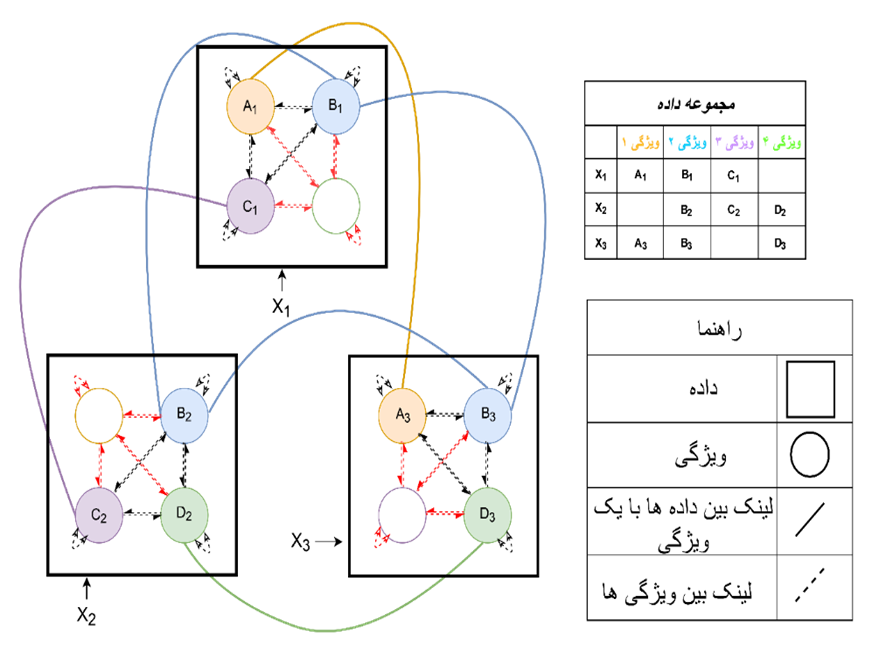
\includegraphics[width=0.94\linewidth]{./img/chap3/missing-features.png}%
  }{%
    \fbox{\parbox{0.86\linewidth}{\centering
      محل تصویر اصلی ویژگی‌های ناموجود؛ فایل \lr{img/chap3/missing-features.png} هنوز به مخزن افزوده نشده است.}}%
  }
  \caption{نمونه‌ای از گراف در حضور ویژگی‌های ناموجود. دایره‌های توخالی محل ویژگی‌های غیرفعال را نشان می‌دهند؛ یال‌های قرمز درون‌نمونه‌ای، انتقال‌های غیرمجاز هستند و در محاسبه احتمال‌های واقعی انتخاب ویژگی شرکت نمی‌کنند.}
  \label{fig:ch3-missing-features}
\end{figure}

علاوه بر محدودیت وجود ویژگی، در تعریف حرکت روی گراف فرض می‌کنیم نمونه آغازین مسیر پس از خروج از آن دوباره بازدید نشود؛ ولی بازدید مجدد از سایر نمونه‌ها مجاز است. بنابراین اگر مسیر از $X_s$ آغاز شود، در مراحل بعدی مقصد $X_s$ از مجموعه مقصدهای قابل انتخاب حذف می‌شود. نحوه نرمال‌سازی سیاست و توزیع انتقال با لحاظ این محدودیت‌ها در بخش‌های بعدی تشریح خواهد شد.

\section{سیاست انتخاب ویژگی وابسته به فرضیه}
\label{sec:ch3-policy}
\subsection{سیاست انتخاب ویژگی در نخستین گام}
\label{subsec:ch3-initial-policy}
برای شروع حرکت از نمونه $X_s$، هنوز ویژگی قبلی وجود ندارد. بنابراین سیاست اولیه را با بردار پارامترهای $\eta^{(c)}\in\mathbb R^m$ و توزیع $\rho^{(c)}$ تعریف می‌کنیم. اگر $B_s^{(0)}$ مجموعه ویژگی‌های موجودی باشد که از طریق آن‌ها می‌توان انتقال معتبری از $X_s$ انجام داد، داریم:
\[
\rho^{(c)}(b\mid X_s)=
\frac{\mathbf1_{\{b\in B_s^{(0)}\}}\exp(\eta_b^{(c)})}
{\sum_{d\in B_s^{(0)}}\exp(\eta_d^{(c)})}.
\]
در نتیجه احتمال اولیه ویژگی‌های ناموجود یا غیرقابل استفاده دقیقاً صفر است. بردار $\eta^{(c)}$ برای تمام مبدأها مشترک است؛ تفاوت توزیع‌های اولیه تنها از محدودیت ویژگی‌های قابل انتخاب و ویژگی‌های موجود هر نمونه ناشی می‌شود.

\subsection{ماتریس گذار ویژگی‌ها و پارامترهای مشترک}
\label{subsec:ch3-policy-matrix}
برای گام‌های بعدی، پارامترهای سیاست کلاس $c$ را در ماتریس
\[
\Theta^{(c)}=[\theta_{ab}^{(c)}]_{m\times m}
\]
قرار می‌دهیم. سطر $a$ انتخاب ویژگی بعدی پس از ویژگی $a$ را توصیف می‌کند. این ماتریس می‌تواند نامتقارن باشد و درایه‌های قطر اصلی آن نیز مجازند؛ بنابراین سیاست هم گذارهای جهت‌دار با وزن‌های متفاوت و هم ادامه حرکت روی همان ویژگی را پوشش می‌دهد. به‌جای ساخت یک ماتریس برای هر نمونه، یک ماتریس سراسری برای هر فرضیه آموزش داده می‌شود. مجموعه کامل پارامترهای سیاست‌ها از مرتبه $O(Km^2)$ است.

\subsection{اعمال محدودیت ویژگی‌های موجود و نرمال‌سازی}
\label{subsec:ch3-policy-mask}
اگر مبدأ مسیر $X_s$ و نمونه فعلی $X_j$ باشد، مجموعه ویژگی‌هایی که واقعاً می‌توانند به مقصدی مجاز منتهی شوند را چنین تعریف می‌کنیم:
\[
B_j^{(-s)}=
\left\{
b\in A_{X_j}:
\sum_{\substack{\ell\in I_b\\\ell\ne j,\ \ell\ne s}}
w_b(X_j,X_\ell)>0
\right\}.
\]
برای $j\ne s$، احتمال انتخاب ویژگی $b$ پس از ویژگی $a$ برابر است با
\[
\pi^{(c,-s)}(b\mid X_j,a)=
\frac{\mathbf1_{\{b\in B_j^{(-s)}\}}\exp(\theta_{ab}^{(c)})}
{\sum_{d\in B_j^{(-s)}}\exp(\theta_{ad}^{(c)})}.
\]
این نرمال‌سازی باید \emph{پس از} اعمال محدودیت انجام شود. در واقع حتی اگر یک درایه $\Theta^{(c)}$ بزرگ باشد، در صورتی که ویژگی مقصد ناموجود یا انتقال نامجاز باشد، احتمال مؤثر آن صفر است. برای نمونه‌هایی با مجموعه ویژگی‌های متفاوت، صورت و مخرج رابطه تغییر می‌کنند؛ اما پارامترهای اصلی همان ماتریس مشترک باقی می‌مانند.

\subsection{قیود و تفسیر احتمالاتی سیاست}
\label{subsec:ch3-policy-properties}
با فرض ناتهی بودن مجموعه‌های مجاز، هر سطر سیاست مؤثر نامنفی است و مجموع احتمال‌های آن یک می‌شود. احتمال انتقال از $a$ به $b$ لزوماً با احتمال انتقال از $b$ به $a$ برابر نیست. همچنین نرمال‌سازی مجدد فقط روی گزینه‌های مجاز انجام می‌شود؛ به‌همین دلیل مقادیر مثبت ماتریس خام، به‌تنهایی به معنای امکان عبور از یال متناظر نیستند. این تفکیک میان «تمایل آموخته‌شده» و «انتقال مجاز»، همان مفهوم یال‌های ممنوع نشان‌داده‌شده در شکل~\ref{fig:ch3-missing-features} است.

\section{حرکت تصادفی چندگامی روی گراف}
\label{sec:ch3-walk}
\subsection{تعریف حالت و ماتریس انتقال}
\label{subsec:ch3-markov-state}
برای آنکه فرایند حرکت خاصیت مارکوفی داشته باشد، حالت را به‌شکل زوج $(X_j,a)$ تعریف می‌کنیم: نمونه فعلی $X_j$ و ویژگی $a$ که در انتقال اخیر استفاده شده است. برای مسیر آغازشده از $X_s$، تنها حالت‌های دارای $j\ne s$ در فضای حالت‌های پس از حرکت اول قرار می‌گیرند. ازاین‌رو نماد $\mathcal U_s$ را برای مجموعه این حالت‌های فعال به کار می‌بریم.

برای $j\ne s$ و ویژگی $b$، توزیع مقصد پس از حذف مبدأ با
\[
T_b^{(-s)}(X_\ell\mid X_j)=
\frac{\mathbf1_{\{\ell\in I_b,\ \ell\ne j,\ \ell\ne s\}}w_b(X_j,X_\ell)}
{\displaystyle\sum_{\substack{h\in I_b\\h\ne j,\ h\ne s}}w_b(X_j,X_h)}
\]
تعریف می‌شود، مشروط بر آنکه مخرج مثبت باشد. شرط کفایت نمونه در بخش~\ref{subsec:ch3-assumptions} معتبر بودن این توزیع را برای ویژگی‌های قابل انتخاب تضمین می‌کند.

\subsection{ترکیب انتخاب ویژگی و جابه‌جایی بین نمونه‌ها}
\label{subsec:ch3-combined-transition}
در هر گام، ابتدا ویژگی بعدی با سیاست $\pi^{(c,-s)}$ انتخاب می‌شود؛ سپس با احتمال $T_b^{(-s)}$ نمونه مقصد تعیین می‌گردد. بنابراین عنصر ماتریس انتقالِ وابسته به مبدأ و فرضیه، برابر است با
\[
M_s^{(c)}((X_j,a),(X_\ell,b))
=\pi^{(c,-s)}(b\mid X_j,a)\,
T_b^{(-s)}(X_\ell\mid X_j).
\]
توزیع اولین حالت بازدیدشده نیز به‌شکل
\[
r_s^{(c)}(X_j,b)
=\rho^{(c)}(b\mid X_s)\,T_b(X_j\mid X_s)
\]
محاسبه می‌شود. در اینجا $T_b(X_j\mid X_s)$ همان انتقال اولیه با ممنوعیت انتخاب خود مبدأ به‌عنوان مقصد است. ماتریس $M_s^{(c)}$ معمولاً برای مبدأهای مختلف یکسان نیست، زیرا حذف مبدأ بر مجموعه مقصدهای مجاز و ضرایب نرمال‌سازی اثر دارد.

\subsection{توقف هندسی و وزن‌دهی به عمق مشاهده}
\label{subsec:ch3-stopping}
پس از هر مشاهده، حرکت با احتمال ثابت $\beta\in(0,1]$ متوقف می‌شود. در حالت بدون محدودیت افق، طول مسیر $L$ دارای توزیع هندسی
\[
\Pr(L=\ell)=\beta(1-\beta)^{\ell-1},
\qquad \ell=1,2,\ldots
\]
است. برای کنترل اهمیت مشاهدات دورتر، ضریب $\lambda\in(0,1]$ را در نظر می‌گیریم؛ وزن خام مشاهده در گام $t$ برابر $\lambda^{t-1}$ است. مقدار $\lambda=1$ به همه مشاهدات هر مسیر وزن یکسان می‌دهد، درحالی‌که مقادیر کوچک‌تر بر همسایگی‌های نزدیک‌تر تأکید می‌کنند. $\beta$ و $\lambda$ در استخراج اولیه، ابرپارامترهای ثابت روش هستند.

\subsection{منع بازگشت به مبدأ و امکان بازدید دوباره از سایر نمونه‌ها}
\label{subsec:ch3-origin-exclusion}
ممنوعیت بازگشت به مبدأ در \emph{تمام} گام‌ها اعمال می‌شود، نه فقط در انتقال اول. این محدودیت به‌خصوص در محاسبه بازنمایی نمونه آموزشی اهمیت دارد، زیرا از مشاهده مستقیم برچسب همان نمونه در طول مسیر آن جلوگیری می‌کند. در عوض، هیچ ممنوعیت کلی برای مراجعه دوباره به سایر نمونه‌ها اعمال نمی‌شود. با فرض وجود انتقال معتبر، حرکت تا زمان توقف تصادفی ادامه دارد و نیازی به تعریف سازوکار جداگانه برای بن‌بست نیست.

\section{استخراج بازنمایی احتمالاتی نمونه‌ها}
\label{sec:ch3-representation}
\subsection{توزیع برچسب در یک گام انتقال}
\label{subsec:ch3-one-step-label}
برای ویژگی $a$ در نمونه فعلی $X_j$، توزیع برچسب‌های قابل مشاهده پس از انتقال را با
\[
Q_{X_j,a}^{(-s)}=
\sum_{\substack{\ell\in I_a\\\ell\ne j,\ \ell\ne s}}
T_a^{(-s)}(X_\ell\mid X_j)\,e_{y_\ell}
\]
نشان می‌دهیم. این بردار در $\Delta^{K-1}$ قرار دارد و صرفاً با برچسب مقصدهای مجاز ساخته می‌شود. توزیع انتخاب ویژگی، این بردارهای یک‌گامی را در طول حرکت با یکدیگر ترکیب می‌کند.

\subsection{بردار نرمال‌شده مشاهدات در یک مسیر}
\label{subsec:ch3-path-representation}
اگر یک مسیر $W$ شامل مشاهده نمونه‌های $X_{j_1},\ldots,X_{j_L}$ باشد، نمایش برچسبی آن را به‌شکل
\[
R(W)=\frac{1}{Z_L(\lambda)}
\sum_{t=1}^{L}\lambda^{t-1}e_{y_{j_t}},
\qquad
Z_L(\lambda)=\sum_{t=1}^{L}\lambda^{t-1}
\]
تعریف می‌کنیم. نرمال‌سازی \emph{برای هر مسیر} انجام می‌شود؛ در نتیجه $\sum_k R_k(W)=1$ و طول‌های متفاوت مسیر موجب تغییر مقیاس بردار حاصل نمی‌شوند. بازنمایی نمونه، امید ریاضی همین بردارهای نرمال‌شده است:
\[
P_{X_s}^{(c)}=\mathbb E_{\pi^{(c)}}[R(W)\mid X_s].
\]
این تعریف با جمع‌زدن وزن‌های بازدیدها روی همه مسیرها و سپس نرمال‌سازی نهایی آن جمع، به‌طور کلی یکسان نیست.

\subsection{امید ریاضی مسیرها و ضرایب تجمیع چندگامی}
\label{subsec:ch3-walk-coefficients}
برای محاسبه تحلیلی، ابتدا فرض می‌کنیم طول حرکت حداکثر $H$ باشد و مسیر باقی‌مانده در گام $H$ متوقف شود. در این صورت
\[
p_\ell=\Pr(L=\ell)=
\begin{cases}
\beta(1-\beta)^{\ell-1},&1\le\ell<H,\\
(1-\beta)^{H-1},&\ell=H.
\end{cases}
\]
ضریب مؤثر مشاهده در عمق $t$ از جابه‌جایی ترتیب امید ریاضی و جمع محدود حاصل می‌شود:
\[
a_t(\beta,\lambda,H)
=\lambda^{t-1}\sum_{\ell=t}^{H}\frac{p_\ell}{Z_\ell(\lambda)}.
\]
این ضرایب مستقل از سیاست‌اند، نامنفی هستند و در مجموع یک می‌شوند؛ زیرا
\[
\sum_{t=1}^{H}a_t
=\sum_{\ell=1}^{H}\frac{p_\ell}{Z_\ell}
\sum_{t=1}^{\ell}\lambda^{t-1}
=\sum_{\ell=1}^{H}p_\ell=1.
\]
بنابراین بازنمایی نهایی همچنان یک توزیع احتمال است. در حالت افق نامحدود نیز می‌توان با جایگزینی کران بالای جمع با بی‌نهایت و با توجه به نامنفی بودن جمله‌ها همین نتیجه را به دست آورد.

\subsection{محاسبه تحلیلی بازنمایی و تقریب مونت‌کارلو}
\label{subsec:ch3-analytic-representation}
ماتریس $Y_s$ را طوری می‌سازیم که سطر متناظر با حالت $(X_j,a)$ برابر $e_{y_j}^{T}$ باشد. با قرار دادن توزیع حالت‌های گام اول $v_{s,1}=r_s^{(c)}$ و بازگشت
\[
v_{s,t+1}=v_{s,t}M_s^{(c)}
\]
توزیع برچسب مشاهده‌شده در گام $t$ برابر $v_{s,t}Y_s$ می‌شود. در نتیجه
\[
\boxed{
P_{X_s}^{(c)}
=\sum_{t=1}^{H}a_t\,r_s^{(c)}
\bigl(M_s^{(c)}\bigr)^{t-1}Y_s.
}
\]
این فرمول امید ریاضی بازنمایی نرمال‌شده مسیر است و به شبیه‌سازی مسیر نیازی ندارد. همچنین می‌توان با نمونه‌گیری مستقل از مسیرهای $W_1,\ldots,W_N$ از برآوردگر
\[
\widehat P_{X_s}^{(c)}
=\frac1N\sum_{\nu=1}^{N}R(W_\nu)
\]
استفاده کرد که برای سیاست و توزیع توقف ثابت، نسبت به $P_{X_s}^{(c)}$ نااریب است. نااریبی بازنمایی نمونه‌گیری‌شده به‌تنهایی به معنای نااریبی امتیازهای غیرخطی محاسبه‌شده از آن نیست.

محاسبه تحلیلی برای ساخت تابع هدف مشتق‌پذیر مناسب است؛ در مقابل، نمونه‌گیری از مسیرها می‌تواند برای ارزیابی تقریبی یا مقیاس‌های بزرگ‌تر مورد استفاده قرار گیرد. در عمل افق $H$ باید بر اساس موازنه دقت و هزینه انتخاب شود. برای مقایسه با حرکت نامحدود، با یک کوپلینگ از مسیرهای مشترک تا گام $H$، خطای نرم یکِ حاصل از توقف اجباری را می‌توان با $2(1-\beta)^H$ از بالا محدود کرد؛ زیرا تنها مسیرهایی که طول طبیعی آن‌ها از $H$ بیشتر است می‌توانند اختلاف ایجاد کنند.

\section{مراکز کلاس‌ها و مبانی اطلاعاتی بازنمایی}
\label{sec:ch3-prototypes}
\subsection{بازنمایی نمونه‌های همه کلاس‌ها تحت یک سیاست}
\label{subsec:ch3-all-class-representation}
برای ارزیابی قدرت تشخیص فرضیه $c$، سیاست $\pi^{(c)}$ را بر روی نمونه‌های تمام کلاس‌ها اجرا می‌کنیم، نه فقط نمونه‌های با برچسب $c$. بدین ترتیب بازنمایی‌های
\[
\mathcal P^{(c)}=\{P_{X_i}^{(c)}\}_{i=1}^{n}
\]
در یک فضای توزیع‌های احتمال مشترک قرار می‌گیرند. این نکته برای یادگیری فرضیه‌ها ضروری است؛ زیرا سیاستی که همه نمونه‌ها را، فارغ از برچسب واقعی آن‌ها، به یک توزیع ثابت نگاشت کند، قادر به رد فرضیه نادرست نخواهد بود؛ حتی اگر توزیع ثابت سیاست‌های کلاس‌های مختلف با هم متفاوت باشد.

\subsection{تعریف مراکز کلاس‌ها به تفکیک فرضیه}
\label{subsec:ch3-centers}
مرکز نمونه‌های دارای برچسب واقعی $k$، تحت سیاست مربوط به فرضیه $c$، به‌شکل
\[
\boxed{
V_{k\mid c}
=\frac{1}{n_k}\sum_{i\in\mathcal C_k}P_{X_i}^{(c)}
}
\]
تعریف می‌شود. پس برای هر سیاست یک مجموعه $K$تایی از مراکز وجود دارد؛ به‌طور مثال $V_{k\mid c}$ و $V_{k\mid d}$ معمولاً برابر نیستند. این وابستگی را نباید با میانگین بازنمایی‌های هر کلاس صرفاً تحت سیاست برچسب واقعی همان کلاس اشتباه گرفت.

\subsection{بهینگی میانگین در واگرایی کولبک--لایبلر}
\label{subsec:ch3-kl-barycenter}
برای توزیع‌های $p,q\in\Delta^{K-1}$، واگرایی کولبک--لایبلر از $p$ به $q$ را با
\[
D_{\mathrm{KL}}(p\Vert q)
=\sum_{h=1}^{K}p_h\log\frac{p_h}{q_h}
\]
نشان می‌دهیم؛ قرارداد $0\log(0/q)=0$ برقرار است و اگر $p_h>0$ ولی $q_h=0$ باشد، واگرایی نامتناهی است.

برای اثبات بهینگی مرکز میانگین، $p_i=P_{X_i}^{(c)}$ و $\bar p=n_k^{-1}\sum_{i\in\mathcal C_k}p_i$ را در نظر بگیریم. برای هر توزیع $q$ با پشتیبان مناسب داریم:
\[
\begin{aligned}
\sum_{i\in\mathcal C_k}D_{\mathrm{KL}}(p_i\Vert q)
&=\sum_{i\in\mathcal C_k}D_{\mathrm{KL}}(p_i\Vert\bar p)
+n_kD_{\mathrm{KL}}(\bar p\Vert q).
\end{aligned}
\]
چون جمله آخر نامنفی است و فقط در $q=\bar p$ صفر می‌شود، مرکز میانگین کمینه‌ساز یکتای مجموع واگرایی‌ها در فضای توزیع‌های مجاز است. این نتیجه \emph{بهینگی میانگین به‌عنوان نمونه‌نمای کلاسی تحت معیار انتخاب‌شده} را اثبات می‌کند؛ اما به معنی کفایت آماری میانگین برای بازسازی تمام توزیع واقعی بازنمایی‌های کلاس نیست.

\subsection{تفسیر مراکز بر اساس درست‌نمایی مشترک}
\label{subsec:ch3-joint-likelihood}
اگر بردارهای $p_i$ را فراوانی نسبی مشاهدات دسته‌ای در نظر بگیریم و فرض کنیم تمام مشاهدات کلاس $k$ از یک توزیع مرجع $q$ پیروی می‌کنند، بخش وابسته به $q$ در لگاریتم درست‌نمایی مشترک متناسب با
\[
\sum_{i\in\mathcal C_k}\sum_{h=1}^{K}p_{i,h}\log q_h
=n_k\sum_{h=1}^{K}\bar p_h\log q_h
\]
است. بیشینه‌سازی این عبارت روی سیمپلکس، همان $q=\bar p$ را نتیجه می‌دهد. این استدلال یک \emph{تفسیر مدل‌مبنای} مراکز است؛ برچسب‌های مشاهدات متوالی یک حرکت روی گراف در حالت کلی مستقل و هم‌توزیع نیستند و نباید مدل دسته‌ای مستقل را یک خاصیت اثبات‌شده آن حرکت تلقی کرد.

\subsection{هموارسازی توزیع‌ها و ملاحظات عددی}
\label{subsec:ch3-center-smoothing}
برای جلوگیری از لگاریتم صفر، در پیاده‌سازی می‌توان مراکز را با
\[
\widetilde V_{k\mid c}
=\frac{V_{k\mid c}+\varepsilon\mathbf1}{1+K\varepsilon},
\qquad\varepsilon>0
\]
هموار کرد. این تبدیل، توزیع را در سیمپلکس نگه می‌دارد و همه مؤلفه‌ها را مثبت می‌کند. اثبات بهینگی میانگین در زیربخش قبل برای مراکز هموارنشده بیان شده است؛ هموارسازی، نسخه تنظیم‌شده‌ای از همان نمونه‌نماست و ممکن است مقدار بهینه واگرایی اولیه را تغییر دهد. مقدار $\varepsilon$ باید کوچک و ثابت یا به‌طور جداگانه اعتبارسنجی شود.

\section{آزمون فرضیه برای تشخیص تعلق به کلاس}
\label{sec:ch3-testing}
\subsection{تعریف فرضیه‌های کلاسی و انواع خطا}
\label{subsec:ch3-hypotheses}
برای هر کلاس $c$، دو فرضیه
\[
H_0^{(c)}:Y=c,\qquad H_1^{(c)}:Y\ne c
\]
تعریف می‌کنیم. مطابق قرارداد انتخاب‌شده، خطای نوع اول \emph{رد اشتباه فرضیه $H_0^{(c)}$} و خطای نوع دوم \emph{پذیرش اشتباه آن در شرایط درست بودن فرضیه مقابل} است. از آنجا که مجموعه مقابل از چند کلاس تشکیل شده، لازم است نوع تجمیع خطای کلاس‌های منفی نیز مشخص شود.

\subsection{حاشیه تصمیم مبتنی بر اختلاف واگرایی‌ها}
\label{subsec:ch3-kl-margin}
با استفاده از مراکز مربوط به یک سیاست واحد، حاشیه نمونه $X$ بین فرضیه $c$ و رقیب $k\ne c$ را تعریف می‌کنیم:
\[
\begin{aligned}
M_{c,k}(X)
&=D_{\mathrm{KL}}(P_X^{(c)}\Vert V_{k\mid c})
-D_{\mathrm{KL}}(P_X^{(c)}\Vert V_{c\mid c})\\
&=(P_X^{(c)})^T
\log\frac{V_{c\mid c}}{V_{k\mid c}}.
\end{aligned}
\]
نسبت و لگاریتم در این رابطه مؤلفه‌ای‌اند و در صورت وجود مؤلفه صفر از مراکز هموار استفاده می‌شود. مقدار مثبت حاشیه نشان می‌دهد بازنمایی نمونه، بر اساس واگرایی انتخاب‌شده، به مرکز $c$ نزدیک‌تر از مرکز رقیب $k$ است.

با فرض مراکز دقیق و غیرهموار، میانگین حاشیه روی نمونه‌های کلاس $c$ برابر
\[
\frac1{n_c}\sum_{i\in\mathcal C_c}M_{c,k}(X_i)
=D_{\mathrm{KL}}(V_{c\mid c}\Vert V_{k\mid c})
\]
و میانگین آن روی نمونه‌های کلاس $k$ برابر
\[
\frac1{n_k}\sum_{i\in\mathcal C_k}M_{c,k}(X_i)
=-D_{\mathrm{KL}}(V_{k\mid c}\Vert V_{c\mid c})
\]
است. این روابط مبنایی برای تفسیر جدایی مراکز فراهم می‌کنند؛ بااین‌حال صرف بزرگ بودن اختلاف میانگین‌ها، به‌تنهایی کنترل خطای تک‌تک نمونه‌ها را تضمین نمی‌کند.

\subsection{امتیاز آزمون و سخت‌ترین کلاس رقیب}
\label{subsec:ch3-test-score}
برای اینکه فرضیه $c$ در برابر تمام رقیب‌ها ارزیابی شود، امتیاز
\[
\boxed{S_c(X)=\min_{k\ne c}M_{c,k}(X)}
\]
را تعریف می‌کنیم. بنابراین مثبت بودن امتیاز یعنی بازنمایی نمونه به مرکز $c$ از تمام مراکز رقیب نزدیک‌تر است. در یادگیری مشتق‌پذیر، کمینه را می‌توان با
\[
S_{c,\gamma}(X)=
-\gamma\log\left(
\sum_{k\ne c}\exp\left[-M_{c,k}(X)/\gamma\right]\right),
\quad\gamma>0
\]
تقریب زد. رابطه
\[
S_c(X)-\gamma\log(K-1)\le S_{c,\gamma}(X)\le S_c(X)
\]
تفاوت این دو امتیاز را محدود می‌کند و با $\gamma\to0^+$ امتیاز هموار به کمینه دقیق همگرا می‌شود. هموارسازی، قاعده امتیازدهی را تغییر می‌دهد؛ بنابراین آستانه باید برای همان امتیازی تنظیم شود که در آزمون استفاده خواهد شد.

\subsection{ناحیه پذیرش فرضیه و آستانه تصمیم}
\label{subsec:ch3-acceptance}
فرضیه کلاس $c$ هنگامی پذیرفته می‌شود که
\[
S_c(X)\ge\tau_c
\]
و در غیر این صورت رد می‌شود. آستانه $\tau_c$ یک پارامتر مستقل از صفر و وابسته به سیاست، هدف خطا و داده‌های کالیبراسیون است؛ مثبت بودن یا نبودن امتیاز به‌تنهایی قاعده نهایی پذیرش را تعیین نمی‌کند. خطاهای جمعیتی متناظر عبارت‌اند از
\[
\alpha_c=\Pr(S_c(X)<\tau_c\mid Y=c),
\]
\[
\varepsilon_c=
\frac1{K-1}\sum_{k\ne c}
\Pr(S_c(X)\ge\tau_c\mid Y=k).
\]
در اینجا سهم کلاس‌های منفی به‌صورت متوازن میانگین گرفته شده است تا فراوانی بیشتر یک کلاس منفی، به‌تنهایی تابع هدف را مسلط نکند. در کاربردهای حساس، به‌جای میانگین می‌توان بیشینه خطای پذیرش بین کلاس‌های منفی را کنترل کرد.

\section{طراحی تابع هدف یادگیری سیاست}
\label{sec:ch3-objective}
\subsection{محدودیت معیارهای مبتنی بر فاصله و درست‌نمایی}
\label{subsec:ch3-objective-motivation}
بیشینه کردن جدایی مراکز، کمینه کردن مجموع فاصله‌های درون‌کلاسی یا کمینه کردن درست‌نمایی منفیِ مبتنی بر نمره‌های فاصله، الزاماً به کمترین تعداد تصمیم اشتباه منجر نمی‌شود. برای مثال، ممکن است سیاست فرضیه $c$ تمام نمونه‌ها را به یک بردار ثابت $v_c$ بفرستد. اگر در یادگیری فقط بازنمایی نمونه‌های دارای برچسب واقعی خودشان مقایسه شوند، بازنمایی‌های ثابت سیاست‌های متفاوت ممکن است در ظاهر کاملاً جدا باشند؛ ولی همین سیاست هنگام مواجهه با نمونه منفی نیز همان $v_c$ را تولید می‌کند و قدرت رد فرضیه نادرست را ندارد. به همین دلیل در این روش، برای آموزش هر سیاست از نمونه‌های مثبت و منفی همان فرضیه استفاده می‌کنیم و معیار هدف را مستقیماً بر خطای پذیرش نادرست بنا می‌گذاریم.

\subsection{کران‌های احتمالاتی خطای آزمون}
\label{subsec:ch3-error-bounds}
کران‌های مبتنی بر گشتاورها می‌توانند رابطه میان مراکز و خطا را روشن کنند. برای نمونه، اگر برای کلاس مثبت $c$، میانگین و واریانس حاشیه $M_{c,k}$ به‌ترتیب $\mu_{c,k}^+$ و $\nu_{c,k}^+$ باشند و $\mu_{c,k}^+>\tau_c$، نامساوی کانتلی نتیجه می‌دهد
\[
\Pr(M_{c,k}<\tau_c\mid Y=c)
\le
\frac{\nu_{c,k}^+}
{\nu_{c,k}^++(\mu_{c,k}^+-\tau_c)^2}.
\]
ازآنجا که رد فرضیه با وجود دست‌کم یک رقیب دارای حاشیه زیر آستانه رخ می‌دهد، می‌توان کران‌های زوجی را با کران اجتماع ترکیب کرد. به‌صورت مشابه، برای نمونه‌های منفی کلاس $k$ که $\mu_{c,k}^-<\tau_c$ دارند، پذیرش فرضیه $c$ مستلزم $M_{c,k}\ge\tau_c$ است و
\[
\Pr(S_c\ge\tau_c\mid Y=k)
\le
\frac{\nu_{c,k}^-}
{\nu_{c,k}^-+(\tau_c-\mu_{c,k}^-)^2}.
\]
کران‌های چرنوف نیز با استفاده از امید نمایی حاشیه‌ها قابل تشکیل‌اند. این کران‌ها برای تحلیل نظری مفیدند، اما ممکن است محافظه‌کارانه باشند و کمینه کردنشان همواره با کمینه کردن خطای تجربی هم‌راستا نباشد؛ ازاین‌رو در ادامه، تابع هدف مستقیماً بر آزمون مقید استوار می‌شود.

\subsection{صورت‌بندی بهینه‌سازی با کنترل خطای نوع اول}
\label{subsec:ch3-np-objective}
اگر $\delta_c\in[0,1)$ حداکثر خطای نوع اول مجاز باشد، مسئله بنیادی یادگیری هر سیاست به‌شکل
\[
\boxed{
\min_{\pi^{(c)},\,\tau_c}\ \varepsilon_c
\qquad
\text{با قید}\quad \alpha_c\le\delta_c
}
\]
تعریف می‌شود. این صورت‌بندی تفسیری از اصل آزمون‌سازی مقید است؛ در اینجا ادعا نمی‌کنیم امتیاز پیشنهادی نسبت درست‌نمایی بهینه توزیع‌های ناشناخته بازنمایی‌هاست. سیاست و امتیاز، خانواده‌ای محدود از آزمون‌های قابل یادگیری را مشخص می‌کنند و بهینه‌سازی درون همین خانواده انجام می‌شود.

\subsection{تعیین آستانه از چندک امتیازهای مثبت}
\label{subsec:ch3-quantile}
برای سیاست ثابت، امتیازهای نمونه‌های مثبت کلاس $c$ را صعودی مرتب می‌کنیم:
\[
s_{(1)}^+\le\cdots\le s_{(n_c)}^+,\qquad
s_i=S_c(X_i).
\]
اگر $r_c=\lfloor n_c\delta_c\rfloor$ باشد، بزرگ‌ترین آستانه‌ای که با قرارداد پذیرش در حالت تساوی، سهم رد نمونه‌های مثبت آموزشی را از $\delta_c$ بیشتر نمی‌کند، برابر است با
\[
\boxed{
q_c=s_{(r_c+1)}^+
}.
\]
در نتیجه تابع هدف تجربی با جایگزینی این آستانه در نرخ پذیرش نادرست منفی‌ها نوشته می‌شود:
\[
\boxed{
J_c(\pi^{(c)})=
\frac1{K-1}\sum_{k\ne c}\frac1{n_k}
\sum_{i\in\mathcal C_k}
\mathbf1\{S_c(X_i)\ge q_c(\pi^{(c)})\}.
}
\]
این معیار نسبت به هر تبدیل اکیداً صعودی و مشترک بر امتیازهای یک سیاست ناورداست، زیرا تنها ترتیب آن‌ها و موقعیتشان نسبت به چندک مثبت اهمیت دارد. اما به دلیل مرتب‌سازی و تابع شاخص، برای بهینه‌سازی مستقیم گرادیانی مناسب نیست.

\subsection{تابع هدف تجربی و تقریب‌های هموار}
\label{subsec:ch3-smooth-surrogates}
برای به‌دست آوردن آستانه هموار، از تابع
$\operatorname{sig}(u)=(1+\exp(-u))^{-1}$
استفاده می‌کنیم و $t_c$ را جواب معادله
\[
\frac1{n_c}\sum_{i\in\mathcal C_c}
\operatorname{sig}\left(\frac{t_c-s_i}{h_q}\right)
=\frac{r_c+1/2}{n_c},
\qquad h_q>0
\]
قرار می‌دهیم. طرف چپ نسبت به $t_c$ پیوسته و اکیداً صعودی است، پس جواب یکتا وجود دارد. برای امتیازهای مثبت متمایز، با $h_q\to0^+$ این آستانه به $q_c$ همگرا می‌شود. این معادله در صورت وجود تساوی‌های گسترده نیز جواب یکتا دارد، هرچند رفتار حدی آن به تساوی‌ها وابسته است.

دو گزینه هموار برای خطای پذیرش منفی‌ها عبارت‌اند از
\[
\widetilde J_c=
\frac1{K-1}\sum_{k\ne c}\frac1{n_k}
\sum_{i\in\mathcal C_k}
\operatorname{sig}\left(\frac{s_i-t_c}{h_e}\right)
\]
و تابع مبتنی بر سافت‌پلاس
\[
L_c^{\mathrm Q}=
\frac1{K-1}\sum_{k\ne c}\frac1{n_k}
\sum_{i\in\mathcal C_k}
\frac{\log(1+\exp((s_i-q_c)/h_e))}{\log2},
\qquad h_e>0.
\]
برای آستانه \emph{دقیق} $q_c$، هر جمله سافت‌پلاس کران بالای شاخص $\mathbf1\{s_i\ge q_c\}$ است. با جایگزینی $q_c$ توسط آستانه هموار $t_c$، این تضمین به‌صورت خودکار به خطای مبتنی بر $q_c$ منتقل نمی‌شود. همچنین سافت‌پلاس در حد $h_e\to0$ تقریب نقطه‌ای تابع شاخص نیست؛ نقش آن یک زیان حاشیه‌محور با گرادیان فعال برای خطاهای بزرگ است. در مقابل سیگموید به شمارش خطا نزدیک‌تر است، اما ممکن است برای نمونه‌های بسیار بد طبقه‌بندی‌شده دچار اشباع گرادیان شود. انتخاب نهایی میان این جانشین‌ها موضوع ارزیابی تجربی است.

\subsection{استانداردسازی امتیازها و ناوردایی نسبت به مقیاس}
\label{subsec:ch3-score-standardization}
برای کاهش حساسیت تابع زیان هموار به مقیاس عددی حاشیه‌ها، می‌توان امتیازهای \emph{نمونه‌های مختلف تحت یک سیاست} را استاندارد کرد:
\[
u_i=\frac{s_i-\bar s_c}{\sigma_c},
\quad
\bar s_c=\frac1n\sum_i s_i,\quad
\sigma_c^2=\frac1n\sum_i(s_i-\bar s_c)^2.
\]
آستانه و تابع زیان هموار سپس بر حسب $u_i$ محاسبه می‌شوند. اگر $\sigma_c>0$ باشد، تبدیل مشترک $s_i\mapsto as_i+b$ با $a>0$ هیچ تغییری در $u_i$ ایجاد نمی‌کند. این استانداردسازی با نرمال کردن فاصله‌های کلاس‌های مختلف \emph{درون هر نمونه} متفاوت است. در حالت فروپاشی همه امتیازها به یک مقدار، $\sigma_c=0$ خواهد شد؛ بنابراین محاسبات باید همراه با راهکار عددی برای این حالت باشند و افزودن ثابت کوچک به مخرج، ناوردایی دقیق را تنها به‌صورت تقریبی حفظ می‌کند.

\section{بهینه‌سازی و الگوریتم آموزش}
\subsection{پارامتری‌سازی قابل یادگیری سیاست‌ها}
\subsection{مشتق بازنمایی ناشی از حرکت چندگامی}
\subsection{مشتق مراکز کلاس‌ها و امتیاز آزمون}
\subsection{مشتق آستانه چندکی و تابع هدف}
\subsection{پس‌انتشار گرادیان در زنجیره انتقال}
\subsection{الگوریتم آموزش سیاست‌های مستقل کلاسی}
\subsection{پیچیدگی زمانی و حافظه‌ای}

\section{استنتاج، اعتبارسنجی و جمع‌بندی}
\subsection{ساخت بازنمایی و ارزیابی فرضیه‌ها برای نمونه جدید}
\subsection{کالیبراسیون آستانه‌ها و کنترل خطای تعمیم}
\subsection{تجمیع نتایج آزمون‌ها برای تصمیم چندکلاسه}
\subsection{محدودیت‌ها و ملاحظات پیاده‌سازی}
\subsection{جمع‌بندی فصل}
